% defer/rcufundamental.tex

\subsection{RCU Fundamentals}
\label{sec:defer:RCU Fundamentals}
\OriginallyPublished{Section}{sec:defer:RCU Fundamentals}{RCU Fundamentals}{Linux Weekly News}{PaulEMcKenney2007WhatIsRCUFundamentally}

RCU is made up of three fundamental mechanisms, the first being
used for insertion, the second being used for deletion, and the third
being used to allow readers to tolerate concurrent insertions and deletions.
Section~\ref{sec:defer:Publish-Subscribe Mechanism}
describes the publish-subscribe mechanism used for insertion,
Section~\ref{sec:defer:Wait For Pre-Existing RCU Readers}
describes how waiting for pre-existing RCU readers enabled deletion,
and
Section~\ref{sec:defer:Maintain Multiple Versions of Recently Updated Objects}
discusses how maintaining multiple versions of recently updated objects
permits concurrent insertions and deletions.
Finally,
Section~\ref{sec:defer:Summary of RCU Fundamentals}
summarizes RCU fundamentals.

\subsubsection{Publish-Subscribe Mechanism}
\label{sec:defer:Publish-Subscribe Mechanism}

% @@@ Slim down presentation, refer to toolsoftrade and memorder.
% @@@ Summarize care and feeding of address dependencies.
% @@@ Mention language/compiler support being a work in progress.

\begin{listing}[tbp]
\begin{VerbatimL}
struct foo {
	int a;
	int b;
	int c;
};
struct foo *gp = NULL;

/* . . . */

p = kmalloc(sizeof(*p), GFP_KERNEL);
p->a = 1;
p->b = 2;
p->c = 3;
gp = p;
\end{VerbatimL}
\caption{Data Structure Publication (Unsafe)}
\label{lst:defer:Data Structure Publication (Unsafe)}
\end{listing}

One key attribute of RCU is the ability to safely scan data, even
though that data is being modified concurrently.
To provide this ability for concurrent insertion,
RCU uses what can be thought of as a publish-subscribe mechanism.
For example, consider an initially \co{NULL} global pointer
\co{gp} that is to be modified to point to a newly allocated
and initialized data structure.
The code fragment shown in
Listing~\ref{lst:defer:Data Structure Publication (Unsafe)}
(with the addition of appropriate locking)
might be used for this purpose.

Unfortunately, there is nothing forcing the compiler and CPU to execute
the last four assignment statements in order.
If the assignment to \co{gp} happens before the initialization
of \co{p} fields, then concurrent readers could see the
uninitialized values.
Memory barriers are required to keep things ordered, but memory barriers
are notoriously difficult to use.
We therefore encapsulate them into a primitive
\co{rcu_assign_pointer()} that has publication semantics.
The last four lines would then be as follows:

\begin{VerbatimN}[samepage=true]
p->a = 1;
p->b = 2;
p->c = 3;
rcu_assign_pointer(gp, p);
\end{VerbatimN}

The \co{rcu_assign_pointer()}
would \emph{publish} the new structure, forcing both the compiler
and the CPU to execute the assignment to \co{gp} \emph{after}
the assignments to the fields referenced by \co{p}.

However, it is not sufficient to only enforce ordering at the
updater, as the reader must enforce proper ordering as well.
Consider for example the following code fragment:

\begin{VerbatimN}[samepage=true]
p = gp;
if (p != NULL) {
	do_something_with(p->a, p->b, p->c);
}
\end{VerbatimN}

Although this code fragment might well seem immune to misordering,
unfortunately, the
DEC Alpha CPU~\cite{PaulMcKenney2005i,PaulMcKenney2005j}
and value-speculation compiler optimizations can, believe it or not,
cause the values of \co{p->a}, \co{p->b}, and
\co{p->c} to be fetched before the value of \co{p}.
This is perhaps easiest to see in the case of value-speculation
compiler optimizations, where the compiler guesses the value
of \co{p}, fetches \co{p->a}, \co{p->b}, and
\co{p->c}, and then fetches the actual value of \co{p}
in order to check whether its guess was correct.
This sort of optimization is quite aggressive, perhaps insanely so,
but does actually occur in the context of profile-driven optimization.

Clearly, we need to prevent this sort of skullduggery on the
part of both the compiler and the CPU.
The \co{rcu_dereference()} primitive uses
whatever memory-barrier instructions and compiler
directives are required for this purpose:\footnote{
	In the Linux kernel, \co{rcu_dereference()} is implemented via
	a volatile cast, and, on DEC Alpha, a memory barrier instruction.
	In the C11 and C++11 standards, \co{memory_order_consume}
	is intended to provide longer-term support for \co{rcu_dereference()},
	but no compilers implement this natively yet.
	(They instead strengthen \co{memory_order_consume} to
	\co{memory_order_acquire}, thus emitting a needless memory-barrier
	instruction on weakly ordered systems.)}

\begin{VerbatimN}[samepage=true]
rcu_read_lock();
p = rcu_dereference(gp);
if (p != NULL) {
	do_something_with(p->a, p->b, p->c);
}
rcu_read_unlock();
\end{VerbatimN}

The \co{rcu_dereference()} primitive can thus be thought of
as \emph{subscribing} to a given value of the specified pointer,
guaranteeing that subsequent dereference operations will see any
initialization that occurred before the corresponding
\co{rcu_assign_pointer()} operation that published that pointer.
The \co{rcu_read_lock()} and \co{rcu_read_unlock()}
calls are absolutely required: they define the extent of the
RCU read-side critical section.
Their purpose is explained in
Section~\ref{sec:defer:Wait For Pre-Existing RCU Readers},
however, they never spin or block, nor do they prevent the
\co{list_add_rcu()} from executing concurrently.
In fact, in non-\co{CONFIG_PREEMPT} kernels, they generate
absolutely no code.

\begin{figure}[tb]
\centering
\resizebox{3in}{!}{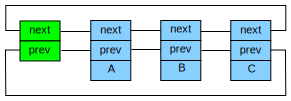
\includegraphics{defer/Linux_list}}
\caption{Linux Circular Linked List}
\label{fig:defer:Linux Circular Linked List}
\end{figure}

\begin{figure}[tb]
\centering
\resizebox{1.8in}{!}{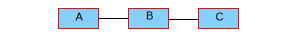
\includegraphics{defer/Linux_list_abbr}}
\caption{Linux Linked List Abbreviated}
\label{fig:defer:Linux Linked List Abbreviated}
\end{figure}

Although \co{rcu_assign_pointer()} and
\co{rcu_dereference()} can in theory be used to construct any
conceivable RCU-protected data structure, in practice it is often better
to use higher-level constructs.
Therefore, the \co{rcu_assign_pointer()} and
\co{rcu_dereference()}
primitives have been embedded in special RCU variants of Linux's
list-manipulation API.
Linux has two variants of doubly linked list, the circular
\co{struct list_head} and the linear
\co{struct hlist_head}/\co{struct hlist_node} pair.
The former is laid out as shown in
Figure~\ref{fig:defer:Linux Circular Linked List},
where the green (leftmost) boxes represent the list header and the blue
(rightmost three) boxes represent the elements in the list.
This notation is cumbersome, and will therefore be abbreviated as shown in
Figure~\ref{fig:defer:Linux Linked List Abbreviated},
which shows only the non-header (blue) elements.

\begin{listing}[tbp]
\begin{linelabel}[ln:defer:RCU Data Structure Publication]
\begin{VerbatimL}[commandchars=\\\[\]]
struct foo {
	struct list_head *list;
	int a;
	int b;
	int c;
};
LIST_HEAD(head);

/* . . . */

p = kmalloc(sizeof(*p), GFP_KERNEL);
p->a = 1;
p->b = 2;
p->c = 3;
list_add_rcu(&p->list, &head);		\lnlbl[add_rcu]
\end{VerbatimL}
\end{linelabel}
\caption{RCU Data Structure Publication}
\label{lst:defer:RCU Data Structure Publication}
\end{listing}

Adapting the pointer-publish example for the linked list results in
the code shown in
Listing~\ref{lst:defer:RCU Data Structure Publication}.

Line~\ref{ln:defer:RCU Data Structure Publication:add_rcu}
must be protected by some synchronization mechanism (most
commonly some sort of lock) to prevent multiple \co{list_add_rcu()}
instances from executing concurrently.
However, such synchronization does not prevent this \co{list_add()}
instance from executing concurrently with RCU readers.

Subscribing to an RCU-protected list is straightforward:

\begin{VerbatimN}[samepage=true]
rcu_read_lock();
list_for_each_entry_rcu(p, head, list) {
	do_something_with(p->a, p->b, p->c);
}
rcu_read_unlock();
\end{VerbatimN}

The \co{list_add_rcu()} primitive publishes an entry, inserting it at
the head of the specified list, guaranteeing that the corresponding
\co{list_for_each_entry_rcu()} invocation will properly subscribe to
this same entry.

\QuickQuiz{}
	What prevents the \co{list_for_each_entry_rcu()} from
	getting a segfault if it happens to execute at exactly the same
	time as the \co{list_add_rcu()}?
\QuickQuizAnswer{
	On all systems running Linux, loads from and stores
	to pointers are atomic, that is, if a store to a pointer occurs at
	the same time as a load from that same pointer, the load will return
	either the initial value or the value stored, never some bitwise
	mashup of the two.
	In addition, the \co{list_for_each_entry_rcu()} always proceeds
	forward through the list, never looking back.
	Therefore, the \co{list_for_each_entry_rcu()} will either see
	the element being added by \co{list_add_rcu()} or it will not,
	but either way, it will see a valid well-formed list.
} \QuickQuizEnd

\begin{figure}[tb]
\centering
\resizebox{3in}{!}{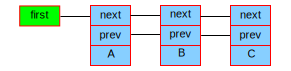
\includegraphics{defer/Linux_hlist}}
\caption{Linux Linear Linked List}
\label{fig:defer:Linux Linear Linked List}
\end{figure}

Linux's other doubly linked list, the hlist,
is a linear list, which means that
it needs only one pointer for the header rather than the two
required for the circular list, as shown in
Figure~\ref{fig:defer:Linux Linear Linked List}.
Thus, use of hlist can halve the memory consumption for the hash-bucket
arrays of large hash tables.
As before, this notation is cumbersome, so hlists will be abbreviated
in the same way lists are, as shown in
Figure~\ref{fig:defer:Linux Linked List Abbreviated}.

\begin{listing}[tbp]
\begin{linelabel}[ln:defer:RCU hlist Publication]
\begin{VerbatimL}[commandchars=\\\[\]]
struct foo {
	struct hlist_node *list;
	int a;
	int b;
	int c;
};
HLIST_HEAD(head);

/* . . . */

p = kmalloc(sizeof(*p), GFP_KERNEL);
p->a = 1;
p->b = 2;
p->c = 3;
hlist_add_head_rcu(&p->list, &head);	\lnlbl[add_head]
\end{VerbatimL}
\end{linelabel}
\caption{RCU {\tt hlist} Publication}
\label{lst:defer:RCU hlist Publication}
\end{listing}

Publishing a new element to an RCU-protected hlist is quite similar
to doing so for the circular list,
as shown in Listing~\ref{lst:defer:RCU hlist Publication}.

As before, line~\ref{ln:defer:RCU hlist Publication:add_head}
must be protected by some sort of synchronization
mechanism, for example, a lock.

Subscribing to an RCU-protected hlist is also similar to the
circular list:

\begin{VerbatimN}[samepage=true]
rcu_read_lock();
hlist_for_each_entry_rcu(p, head, list) {
	do_something_with(p->a, p->b, p->c);
}
rcu_read_unlock();
\end{VerbatimN}

\begin{table*}[tb]
\renewcommand*{\arraystretch}{1.2}
\centering
\footnotesize\OneColumnHSpace{-0.4in}
\begin{tabular}{llll}
\toprule
Category  & Publish	& Retract	& Subscribe \\
\midrule
Pointers  & \tco{rcu_assign_pointer()}
			& \tco{rcu_assign_pointer(..., NULL)}
					& \tco{rcu_dereference()} \\
\midrule
Lists     & \parbox[c][0.37in][c]{1.3in}{
		\co{list_add_rcu()} \\
		\co{list_add_tail_rcu()} \\
		\co{list_replace_rcu()} }
			& \tco{list_del_rcu()}
					& \tco{list_for_each_entry_rcu()} \\
\midrule
Hlists    & \parbox[c][0.5in][c]{1.3in}{
		\co{hlist_add_behind_rcu()} \\
		\co{hlist_add_before_rcu()} \\
		\co{hlist_add_head_rcu()} \\
		\co{hlist_replace_rcu()} }
			& \tco{hlist_del_rcu()}
					& \tco{hlist_for_each_entry_rcu()} \\
\bottomrule
\end{tabular}
\caption{RCU Publish and Subscribe Primitives}
\label{tab:defer:RCU Publish and Subscribe Primitives}
\end{table*}

The set of RCU publish and subscribe primitives are shown in
Table~\ref{tab:defer:RCU Publish and Subscribe Primitives},
along with additional primitives to ``unpublish'', or retract.

Note that the \co{list_replace_rcu()}, \co{list_del_rcu()},
\co{hlist_replace_rcu()}, and \co{hlist_del_rcu()}
APIs add a complication.
When is it safe to free up the data element that was replaced or
removed?
In particular, how can we possibly know when all the readers
have released their references to that data element?

These questions are addressed in the following section.

\subsubsection{Wait For Pre-Existing RCU Readers}
\label{sec:defer:Wait For Pre-Existing RCU Readers}

In its most basic form, RCU is a way of waiting for things to finish.
Of course, there are a great many other ways of waiting for things to
finish, including reference counts, reader-writer locks, events, and so on.
The great advantage of RCU is that it can wait for each of
(say) 20,000 different things without having to explicitly
track each and every one of them, and without having to worry about
the performance degradation, scalability limitations, complex deadlock
scenarios, and memory-leak hazards that are inherent in schemes
using explicit tracking.

In RCU's case, each of the things waited on is called an
\emph{RCU read-side critical section}.
As hinted at in
Section~\ref{sec:defer:Toy Implementation}, an RCU read-side critical
section starts with an \co{rcu_read_lock()} primitive, and ends with a
corresponding \co{rcu_read_unlock()} primitive.
RCU read-side critical sections can be nested, and may contain pretty
much any code, as long as that code does not contain a quiescent state,
for example, within the Linux kernel, it is illegal to sleep within
an RCU read-side critical section because a context switch is a quiescent
state.\footnote{
	However, a special form of RCU called SRCU~\cite{PaulEMcKenney2006c}
	does permit general sleeping in SRCU read-side critical sections.}
If you abide by these conventions, you can use RCU to wait for \emph{any}
pre-existing RCU read-side critical section to complete, and
\co{synchronize_rcu()} does the actual waiting.

% @@@ citations? @@@ RCU accomplishes this feat by indirectly determining
% when these other things have finished~\cite{PaulEMcKenney2007whatisRCU,
% PaulEMcKenney2007PreemptibleRCU}.

\begin{figure}[tb]
\centering
\resizebox{3in}{!}{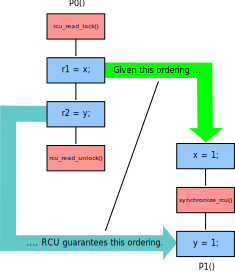
\includegraphics{defer/RCUGuaranteeFwd}}
\caption{RCU Reader and Later Grace Period}
\label{fig:defer:RCU Reader and Later Grace Period}
\end{figure}

The relationship between an RCU read-side critical section and a later
RCU grace period is an if-then relationship, as illustrated by
Figure~\ref{fig:defer:RCU Reader and Later Grace Period}.
If any portion of a given critical section precedes the beginning of
a given grace period, then RCU guarantees that all of that critical
section will precede the end of that grace period.
In the figure, because \co{P0()}'s access to \co{y} precedes
\co{P1()}'s access to this same variable, it is guaranteed that
\co{P0()}'s access to \co{x} will precede \co{P1()}'s access.
In this case, if \co{y}'s final value is 2, then \co{x}'s
final value is guaranteed to also be 2.

\QuickQuiz{}
	What other final values of \co{x} and \co{y} are possible in
	Figure~\ref{fig:defer:RCU Reader and Later Grace Period}?
\QuickQuizAnswer{
	The \co{x == 2 && y == 2} possibility was called out in the text.
	Given that \co{y == 2} implies \co{x == 2}, we know that
	\co{x == 1 && y == 2} is forbidden.
	The following discussion will show that both
	\co{x == 1 && y == 1} and \co{x == 2 && y == 1} are possible.
} \QuickQuizEnd

\begin{figure}[tb]
\centering
\resizebox{3in}{!}{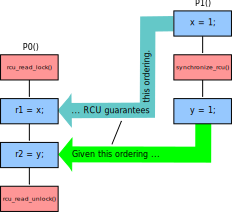
\includegraphics{defer/RCUGuaranteeRev}}
\caption{RCU Reader and Earlier Grace Period}
\label{fig:defer:RCU Reader and Earlier Grace Period}
\end{figure}

The relationship between an RCU read-side critical section and an earlier
RCU grace period is also an if-then relationship, as illustrated by
Figure~\ref{fig:defer:RCU Reader and Earlier Grace Period}.
If any portion of a given critical section follows the end of
a given grace period, then RCU guarantees that all of that critical
section will follow the beginning of that grace period.
In the figure, because \co{P0()}'s access to \co{x} follows
\co{P1()}'s access to this same variable, it is guaranteed that
\co{P0()}'s access to \co{y} will precede \co{P1()}'s access.
In this case, if \co{x}'s final value is 1, then \co{y}'s
final value is guaranteed to also be 1.

\begin{figure}[tb]
\centering
\resizebox{3in}{!}{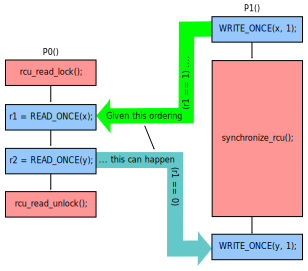
\includegraphics{defer/RCUGuaranteeMid}}
\caption{RCU Reader Within Grace Period}
\label{fig:defer:RCU Reader Within Grace Period}
\end{figure}

Finally, as shown in
Figure~\ref{fig:defer:RCU Reader Within Grace Period},
an RCU read-side critical section can be completely overlapped by
an RCU grace period.
In this case, \co{x}'s final value is 1 and \co{y}'s final value is 2.

However, it cannot be the case that \co{x}'s final value is 2 and \co{y}'s
final value is 1.
This would mean that an RCU read-side critical section had completely
overlapped a grace period, which is forbidden.
RCU's wait-for-readers guarantee therefore has two parts:
(1)~If any part of a given RCU read-side critical section precedes
the beginning of a given grace period, then the entirety of that
critical section precedes the end of that grace period.
(2)~If any part of a given RCU read-side critical section follows
the end of a given grace period, then the entirety of that
critical section follows the beginning of that grace period.
This definition is sufficient for almost all RCU-based algorithms, but
for those wanting more,
simple executable formal models of RCU are available
as part of Linux kernel v4.17 and later, as discussed in
Section~\ref{sec:formal:Axiomatic Approaches and RCU}.
In addition, RCU's ordering properties are examined in much
greater detail in Section~\ref{sec:memorder:RCU}.

Although RCU's wait-for-readers capability really is sometimes used to
order the assignment of values to variables as shown in
Figures~\ref{fig:defer:RCU Reader and Later Grace Period}-\ref{fig:defer:RCU Reader Within Grace Period},
it is more frequently used to safely free data elements removed from
a linked structure, as was done in
Section~\ref{sec:defer:Introduction to RCU}.
The general process is illustrated by the following pseudocode:

\begin{enumerate}
\item	Make a change, for example, remove an element from a linked list.
\item	Wait for all pre-existing RCU read-side critical sections to
	completely finish (for example, by using
	\co{synchronize_rcu()}).
\item	Clean up, for example, free the element that was replaced above.
\end{enumerate}

Given that RCU readers can make forward progress while this update
is in progress, different readers might disagree about the state
of the data structure, a topic taken up by the next section.

\subsubsection{Maintain Multiple Versions of Recently Updated Objects}
\label{sec:defer:Maintain Multiple Versions of Recently Updated Objects}

This section demonstrates how RCU maintains multiple versions of
lists to accommodate synchronization-free readers.
Two examples are presented showing how an element
that might be referenced by a given reader must remain intact
while that reader remains in its RCU read-side critical section.
The first example demonstrates deletion of a list element,
and the second example demonstrates replacement of an element.

\paragraph{Example 1: Maintaining Multiple Versions During Deletion}
\label{sec:defer:Example 1: Maintaining Multiple Versions During Deletion}

We can now revisit the deletion example from
Section~\ref{sec:defer:Introduction to RCU},
but now with the benefit of a firm understanding of the fundamental
concepts underlying RCU.
% @@@ \begin{lineref}[ln:defer:Canonical RCU Replacement Example]
% @@@ To begin this new version of the deletion example,
% @@@ we will modify
% @@@ lines~\lnref{search}-\lnref{kfree} in
% @@@ Listing~\ref{lst:defer:Canonical RCU Replacement Example}
% @@@ to read as follows:
% @@@ \end{lineref}

\begin{linelabel}[ln:defer:RCU Deletion From Linked List]
\begin{VerbatimN}[samepage=true,commandchars=\\\[\]]
p = search(head, key);
if (p != NULL) {
	list_del_rcu(&p->list);		\lnlbl[del_rcu]
	synchronize_rcu();		\lnlbl[sync_rcu]
	kfree(p);
}
\end{VerbatimN}
\end{linelabel}

\begin{figure}[tb]
\centering
\resizebox{3in}{!}{\includegraphics{defer/RCUDeletion}}
\caption{RCU Deletion From Linked List}
\label{fig:defer:RCU Deletion From Linked List}
\end{figure}

This code will update the list as shown in
Figure~\ref{fig:defer:RCU Deletion From Linked List}.
The triples in each element represent the values of fields \co{a},
\co{b}, and \co{c}, respectively.
The red-shaded elements
indicate that RCU readers might be holding references to them,
so in the initial state at the top of the diagram, all elements
are shaded red.
Please note that
we have omitted the backwards pointers and the link from the tail
of the list to the head for clarity.

\begin{lineref}[ln:defer:RCU Deletion From Linked List]
After the \co{list_del_rcu()} on
line~\lnref{del_rcu} has completed, the \co{5,6,7}~element
has been removed from the list, as shown in the second row of
Figure~\ref{fig:defer:RCU Deletion From Linked List}.
Since readers do not synchronize directly with updaters,
readers might be concurrently scanning this list.
These concurrent readers might or might not see the newly removed element,
depending on timing.
However, readers that were delayed (e.g., due to interrupts, ECC memory
errors, or, in \co{CONFIG_PREEMPT_RT} kernels, preemption)
just after fetching a pointer to the newly removed element might
see the old version of the list for quite some time after the
removal.
Therefore, we now have two versions of the list, one with element
\co{5,6,7} and one without.
The \co{5,6,7}~element in the second row of the figure is now
shaded yellow, indicating
that old readers might still be referencing it, but that new
readers cannot obtain a reference to it.

Please note that readers are not permitted to maintain references to
element~\co{5,6,7} after exiting from their RCU read-side
critical sections.
Therefore,
once the \co{synchronize_rcu()} on
line~\lnref{sync_rcu} completes, so that all pre-existing readers are
guaranteed to have completed,
there can be no more readers referencing this
element, as indicated by its green shading on the third row of
Figure~\ref{fig:defer:RCU Deletion From Linked List}.
We are thus back to a single version of the list.
\end{lineref}

At this point, the \co{5,6,7}~element may safely be
freed, as shown on the final row of
Figure~\ref{fig:defer:RCU Deletion From Linked List}.
At this point, we have completed the deletion of
element~\co{5,6,7}.
The following example covers replacement.

\paragraph{Example 2: Maintaining Multiple Versions During Replacement}
\label{sec:defer:Example 2: Maintaining Multiple Versions During Replacement}

To start the replacement example,
here are the last few lines of the
example shown in
% @@@ Listing~\ref{lst:defer:Canonical RCU Replacement Example}:

\begin{linelabel}[ln:defer:Canonical RCU Replacement Example (2nd)]
\begin{VerbatimN}[samepage=true,commandchars=\\\[\],firstnumber=15]
q = kmalloc(sizeof(*p), GFP_KERNEL);	\lnlbl[kmalloc]
*q = *p;				\lnlbl[copy]
q->b = 2;				\lnlbl[update1]
q->c = 3;				\lnlbl[update2]
list_replace_rcu(&p->list, &q->list);	\lnlbl[replace]
synchronize_rcu();			\lnlbl[sync_rcu]
kfree(p);				\lnlbl[kfree]
\end{VerbatimN}
\end{linelabel}

\begin{figure}[tbp]
\centering
\resizebox{2.7in}{!}{\includegraphics{defer/RCUReplacement}}
\caption{RCU Replacement in Linked List}
\label{fig:defer:RCU Replacement in Linked List}
\end{figure}

The initial state of the list, including the pointer \co{p},
is the same as for the deletion example, as shown on the
first row of
Figure~\ref{fig:defer:RCU Replacement in Linked List}.

As before,
the triples in each element represent the values of fields \co{a},
\co{b}, and \co{c}, respectively.
The red-shaded elements might be referenced by readers,
and because readers do not synchronize directly with updaters,
readers might run concurrently with this entire replacement process.
Please note that
we again omit the backwards pointers and the link from the tail
of the list to the head for clarity.

The following text describes how to replace the \co{5,6,7} element
with \co{5,2,3} in such a way that any given reader sees one of these
two values.

\begin{lineref}[ln:defer:Canonical RCU Replacement Example (2nd)]
Line~\lnref{kmalloc} \co{kmalloc()}s a replacement element, as follows,
resulting in the state as shown in the second row of
Figure~\ref{fig:defer:RCU Replacement in Linked List}.
At this point, no reader can hold a reference to the newly allocated
element (as indicated by its green shading), and it is uninitialized
(as indicated by the question marks).

Line~\lnref{copy} copies the old element to the new one, resulting in the
state as shown in the third row of
Figure~\ref{fig:defer:RCU Replacement in Linked List}.
The newly allocated element still cannot be referenced by readers, but
it is now initialized.

Line~\lnref{update1} updates \co{q->b} to the value ``2'', and
line~\lnref{update2} updates \co{q->c} to the value ``3'',
as shown on the fourth row of
Figure~\ref{fig:defer:RCU Replacement in Linked List}.

Now, line~\lnref{replace} does the replacement, so that the new element is
finally visible to readers, and hence is shaded red, as shown on
the fifth row of
Figure~\ref{fig:defer:RCU Replacement in Linked List}.
At this point, as shown below, we have two versions of the list.
Pre-existing readers might see the \co{5,6,7} element (which is
therefore now shaded yellow), but
new readers will instead see the \co{5,2,3} element.
But any given reader is guaranteed to see some well-defined list.

After the \co{synchronize_rcu()} on line~\lnref{sync_rcu} returns,
a grace period will have elapsed, and so all reads that started before the
\co{list_replace_rcu()} will have completed.
In particular, any readers that might have been holding references
to the \co{5,6,7} element are guaranteed to have exited
their RCU read-side critical sections, and are thus prohibited from
continuing to hold a reference.
Therefore, there can no longer be any readers holding references
to the old element, as indicated its green shading in the sixth row of
Figure~\ref{fig:defer:RCU Replacement in Linked List}.
As far as the readers are concerned, we are back to having a single version
of the list, but with the new element in place of the old.

After the \co{kfree()} on line~\lnref{kfree} completes, the list will
appear as shown on the final row of
Figure~\ref{fig:defer:RCU Replacement in Linked List}.
\end{lineref}

Despite the fact that RCU was named after the replacement case,
the vast majority of RCU usage within the Linux kernel relies on
the simple deletion case shown in
Section~\ref{sec:defer:Maintain Multiple Versions of Recently Updated Objects}.

\paragraph{Discussion}
\label{sec:defer:Discussion}

These examples assumed that a mutex was held across the entire
update operation, which would mean that there could be at most two
versions of the list active at a given time.

\QuickQuiz{}
	How would you modify the deletion example to permit more than two
	versions of the list to be active?
\QuickQuizAnswer{
	One way of accomplishing this is as shown in
	Listing~\ref{lst:defer:Concurrent RCU Deletion}.

\begin{listing}[htbp]
\begin{VerbatimL}
spin_lock(&mylock);
p = search(head, key);
if (p == NULL)
	spin_unlock(&mylock);
else {
	list_del_rcu(&p->list);
	spin_unlock(&mylock);
	synchronize_rcu();
	kfree(p);
}
\end{VerbatimL}
\caption{Concurrent RCU Deletion}
\label{lst:defer:Concurrent RCU Deletion}
\end{listing}

	Note that this means that multiple concurrent deletions might be
	waiting in \co{synchronize_rcu()}.
} \QuickQuizEnd

\QuickQuiz{}
	How many RCU versions of a given list can be
	active at any given time?
\QuickQuizAnswer{
	That depends on the synchronization design.
	If a semaphore protecting the update is held across the grace period,
	then there can be at most two versions, the old and the new.

	However, suppose that only the search, the update, and the
	\co{list_replace_rcu()} were protected by a lock, so that
	the \co{synchronize_rcu()} was outside of that lock, similar
	to the code shown in
	Listing~\ref{lst:defer:Concurrent RCU Deletion}.
	Suppose further that a large number of threads undertook an
	RCU replacement at about the same time, and that readers
	are also constantly traversing the data structure.

	Then the following sequence of events could occur, starting from
	the end state of
	Figure~\ref{fig:defer:RCU Replacement in Linked List}:

	\begin{enumerate}
	\item	Thread~A traverses the list, obtaining a reference to
		the 5,2,3 element.
	\item	Thread~B replaces the 5,2,3 element with a new
		5,2,4 element, then waits for its \co{synchronize_rcu()}
		call to return.
	\item	Thread~C traverses the list, obtaining a reference to
		the 5,2,4 element.
	\item	Thread~D replaces the 5,2,4 element with a new
		5,2,5 element, then waits for its \co{synchronize_rcu()}
		call to return.
	\item	Thread~E traverses the list, obtaining a reference to
		the 5,2,5 element.
	\item	Thread~F replaces the 5,2,5 element with a new
		5,2,6 element, then waits for its \co{synchronize_rcu()}
		call to return.
	\item	Thread~G traverses the list, obtaining a reference to
		the 5,2,6 element.
	\item	And the previous two steps repeat quickly, so that all
		of them happen before any of the \co{synchronize_rcu()}
		calls return.
	\end{enumerate}

	Thus, there can be an arbitrary number of versions active,
	limited only by memory and by how many updates could be completed
	within a grace period.
	But please note that data structures that are updated so frequently
	probably are not good candidates for RCU.
	That said, RCU can handle high update rates when necessary.
} \QuickQuizEnd

This sequence of events shows how RCU updates use multiple versions
to safely carry out changes in presence of concurrent readers.
Of course, some algorithms cannot gracefully handle multiple versions.
There are techniques
for adapting such algorithms to RCU~\cite{PaulEdwardMcKenneyPhD},
but these are beyond the scope of this section.

\subsubsection{Summary of RCU Fundamentals}
\label{sec:defer:Summary of RCU Fundamentals}

This section has described the three fundamental components of RCU-based
algorithms:

\begin{enumerate}
\item	a publish-subscribe mechanism for adding new data,

\item	a way of waiting for pre-existing RCU readers to finish,\footnote{
		This component is described in much greater detail in
		Section~\ref{sec:memorder:RCU}.}
	and

\item	a discipline of maintaining multiple versions to permit
	change without harming or unduly delaying concurrent RCU readers.
\end{enumerate}

\QuickQuiz{}
	How can RCU updaters possibly delay RCU readers, given that the
	\co{rcu_read_lock()} and \co{rcu_read_unlock()}
	primitives neither spin nor block?
\QuickQuizAnswer{
	The modifications undertaken by a given RCU updater will cause the
	corresponding CPU to invalidate cache lines containing the data,
	forcing the CPUs running concurrent RCU readers to incur expensive
	cache misses.
	(Can you design an algorithm that changes a data structure
	\emph{without}
	inflicting expensive cache misses on concurrent readers?
	On subsequent readers?)
} \QuickQuizEnd

These three RCU components
allow data to be updated in face of concurrent readers, and
can be combined in different ways to
implement a surprising variety of different types of RCU-based algorithms,
some of which are described in the following section.
